\documentclass[aspectratio=169]{beamer}
\usetheme{Warsaw}

\usepackage{graphicx}
\usepackage[english, russian]{babel}
\usepackage{fontspec}
\usepackage{tikz}

\setbeamercovered{invisible}

% Настройки шрифта
\setsansfont{Cascadia Code} % Основной шрифт
\setmonofont{Monospace}[
Scale=0.9,
Path=./fonts/,
Extension=.ttf
]

\title{КТЗС.КП.КС312.22 ПЗ}
\author{Старостин Г.М.}
\begin{document}
	
\begin{frame}
	\centering
	 % Верхняя часть
	 \begin{center}
		Бюджетное профессиональное образовательное учреждение\\
		<<Омский авиационный колледж имени Н.Е. Жуковского>>
	 \end{center}
	 
	 \vspace{1cm}
	 
	 \parbox{0.8\textwidth}{ 
	 	\fontsize{18}{19}\selectfont
	 	\centering
	 	Проектирование компьютерной\\
	 	сети компании <<Зевс>>
	 }
	 \vspace{2cm}
	 \begin{flushleft}
	 	Студент: Старостин Г.М. \\
	 	Руководитель: Адринский И.Г.
	 \end{flushleft}
	 \vspace{0.5cm}
	 \text{2025 г.}
\end{frame}
	
\begin{frame}{Цели и задачи}
	\begin{block}{\large Цель}
		\begin{itemize}
			\item Создать сеть, основываясь на ТЗ клиента
		\end{itemize}
	\end{block}
	
	\vspace{0.5cm}
	
	\begin{block}{\large Задачи:}
		\begin{itemize}
			\item Провести анализ объекта
			\item Подобрать сетевое оборудование
			\item Разработать схему сети
			\item Рассчитать стоимость инфраструктуры сети
		\end{itemize}
	\end{block}
	
\end{frame}

\begin{frame}{Исходные данные}
	\begin{itemize}
		\item Предполагается установка стойки с сетевым оборудованием и сервера.
		\item Пропускная способность сети не должны быть менее 150 Mb/c.
		\item Проектирование размещения оборудования в стойке и выбор технологий функционирования компьютерной сети заказчик оставляет за исполнителем.
		\item Предоставлена схема этажа здания
	\end{itemize}
\end{frame}

\begin{frame}
	\frametitle{Исходная схема}
	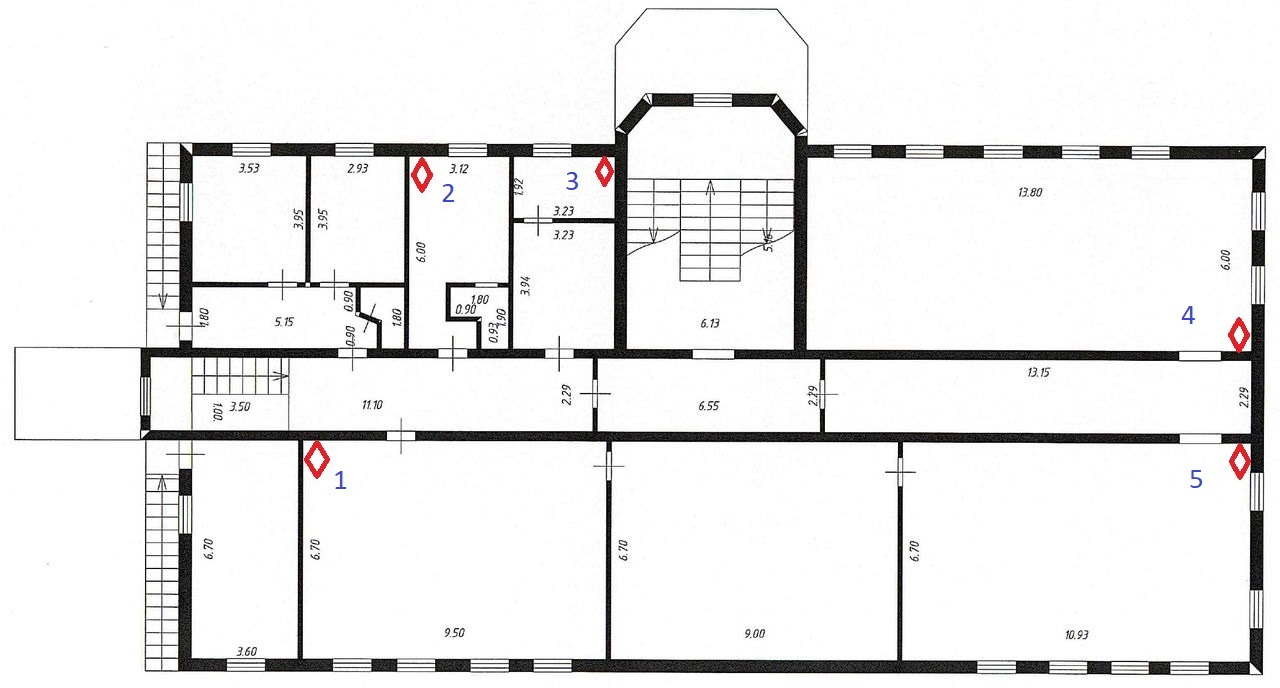
\includegraphics[width=\linewidth]{images/Исходная схема.jpg}
\end{frame}

\begin{frame}{Рабочие места}
	\begin{columns}[T]
		\begin{column}{0.48\textwidth}
			\centering
			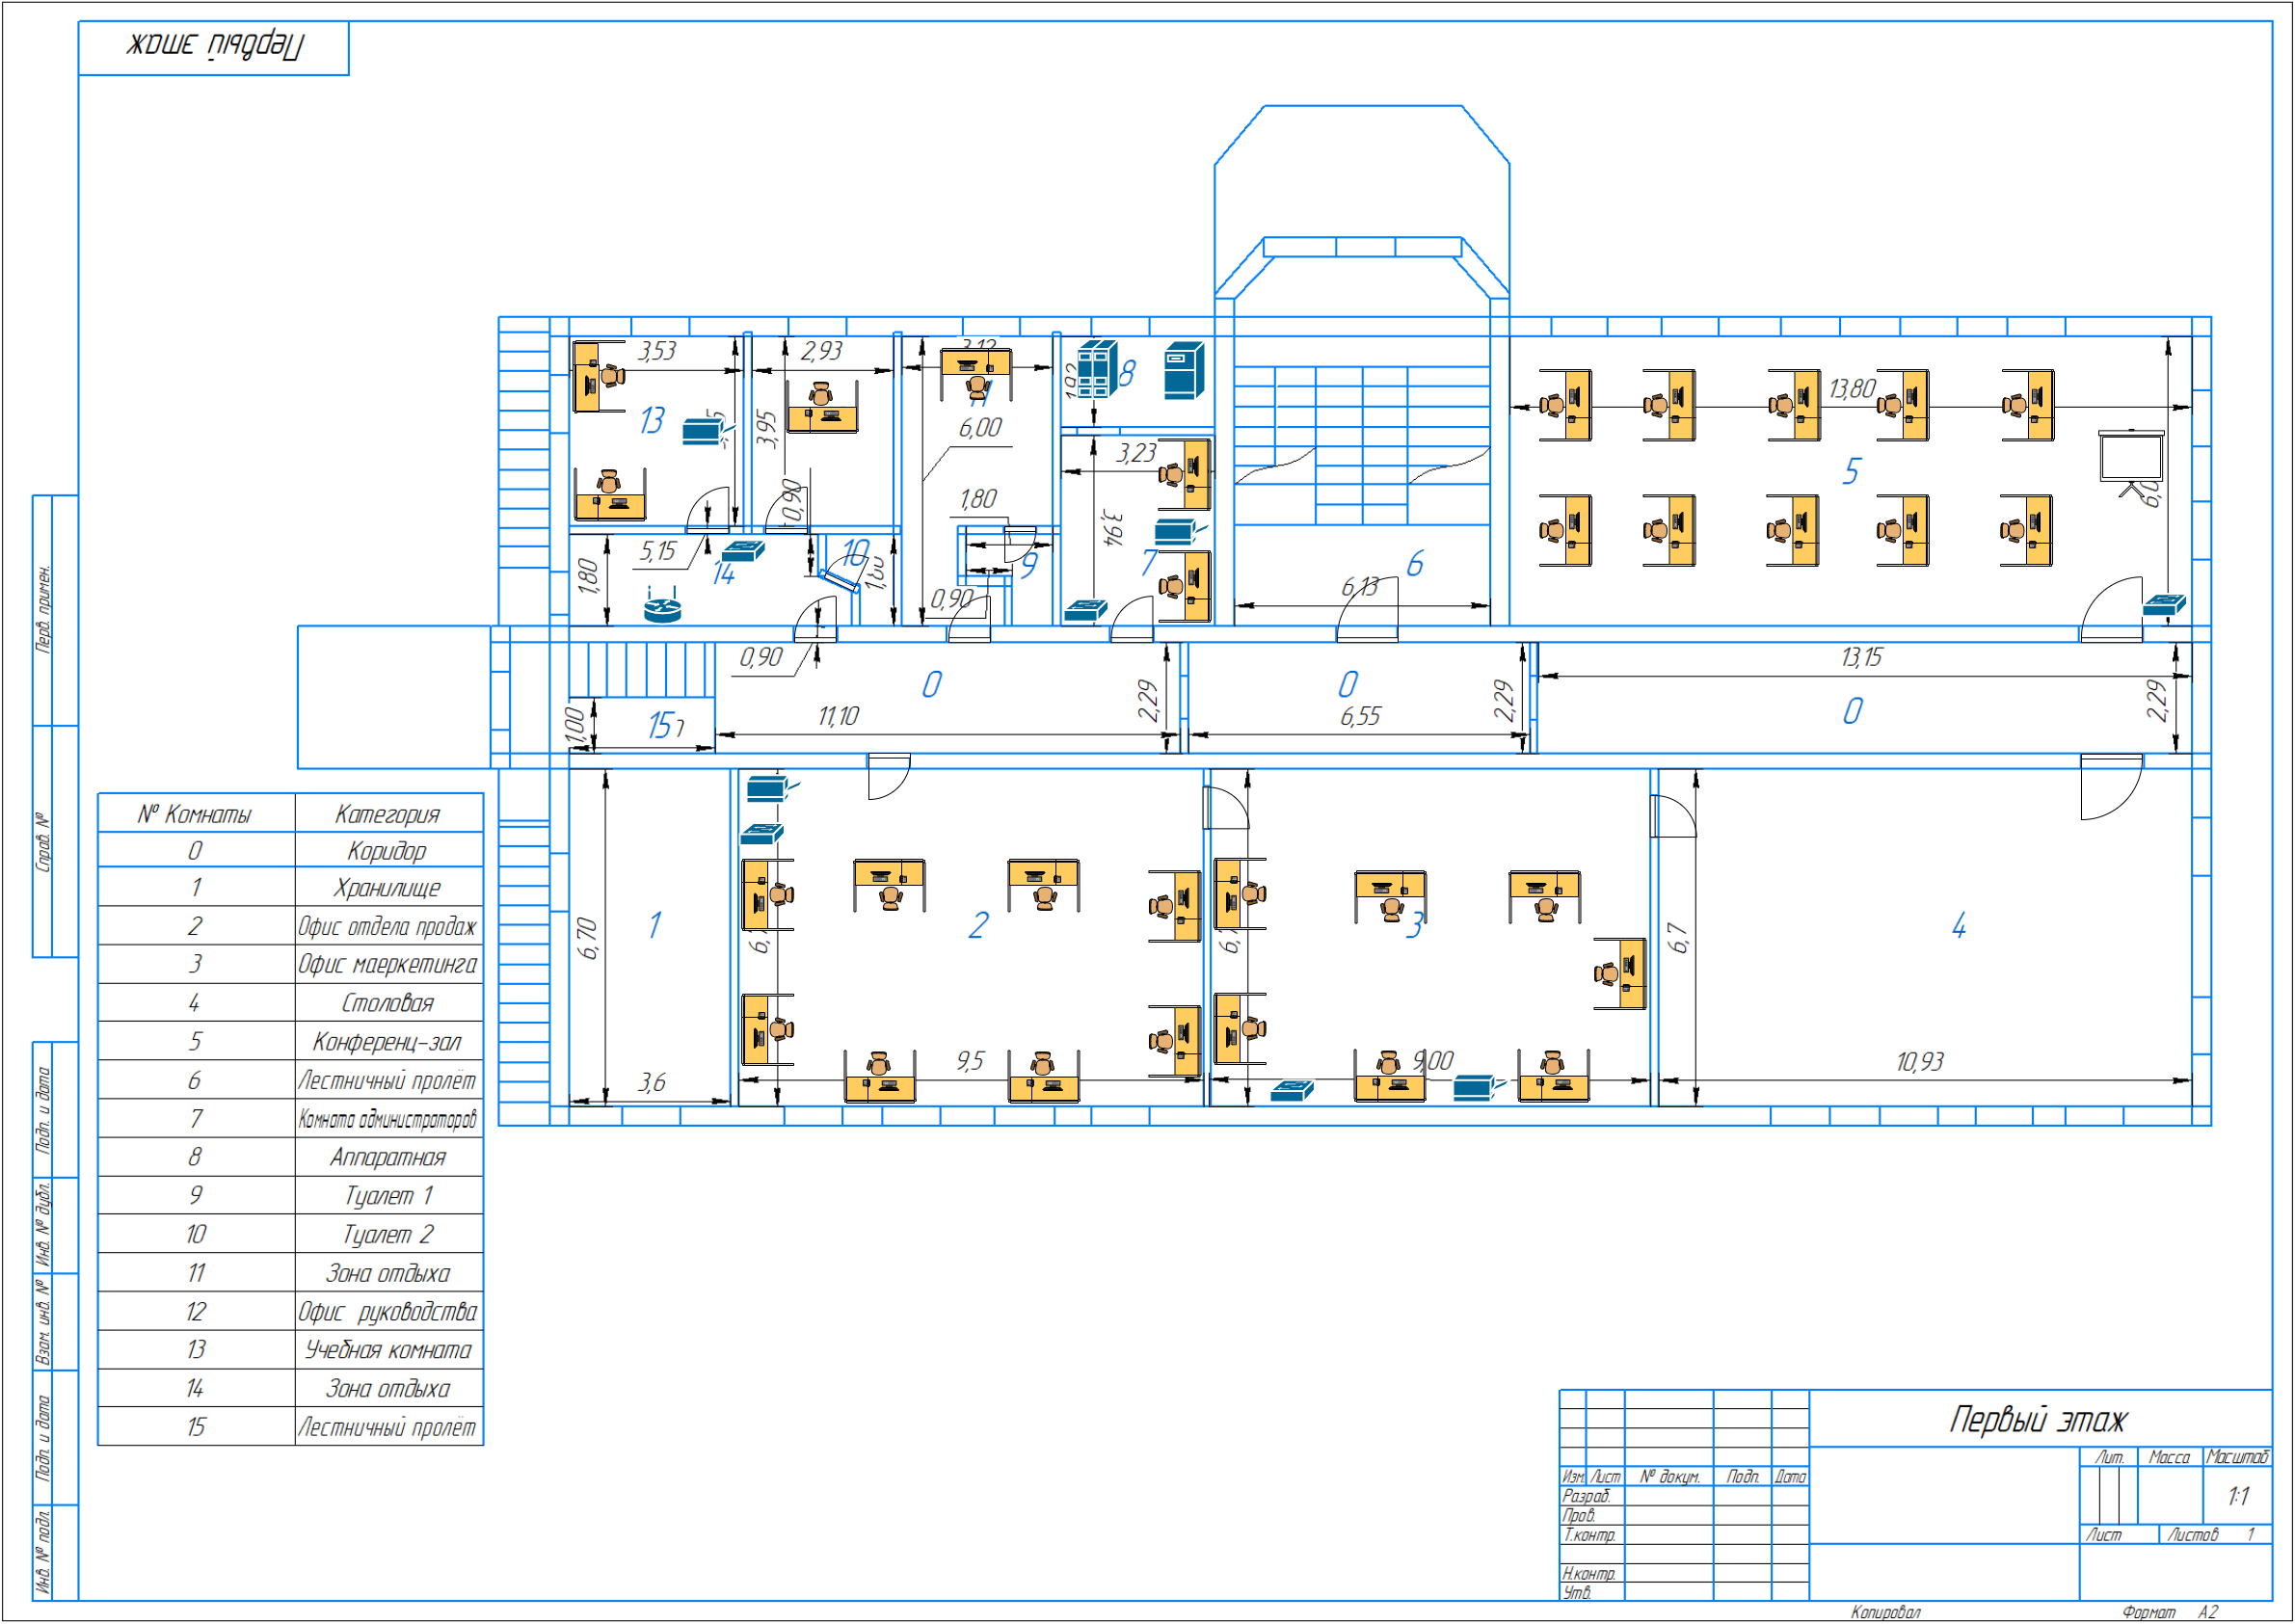
\includegraphics[width=\linewidth]{images/Схема по курсовому(1 этаж).png}
			\text Первый этаж
		\end{column}
		
		\begin{column}{0.48\textwidth}
			\centering
			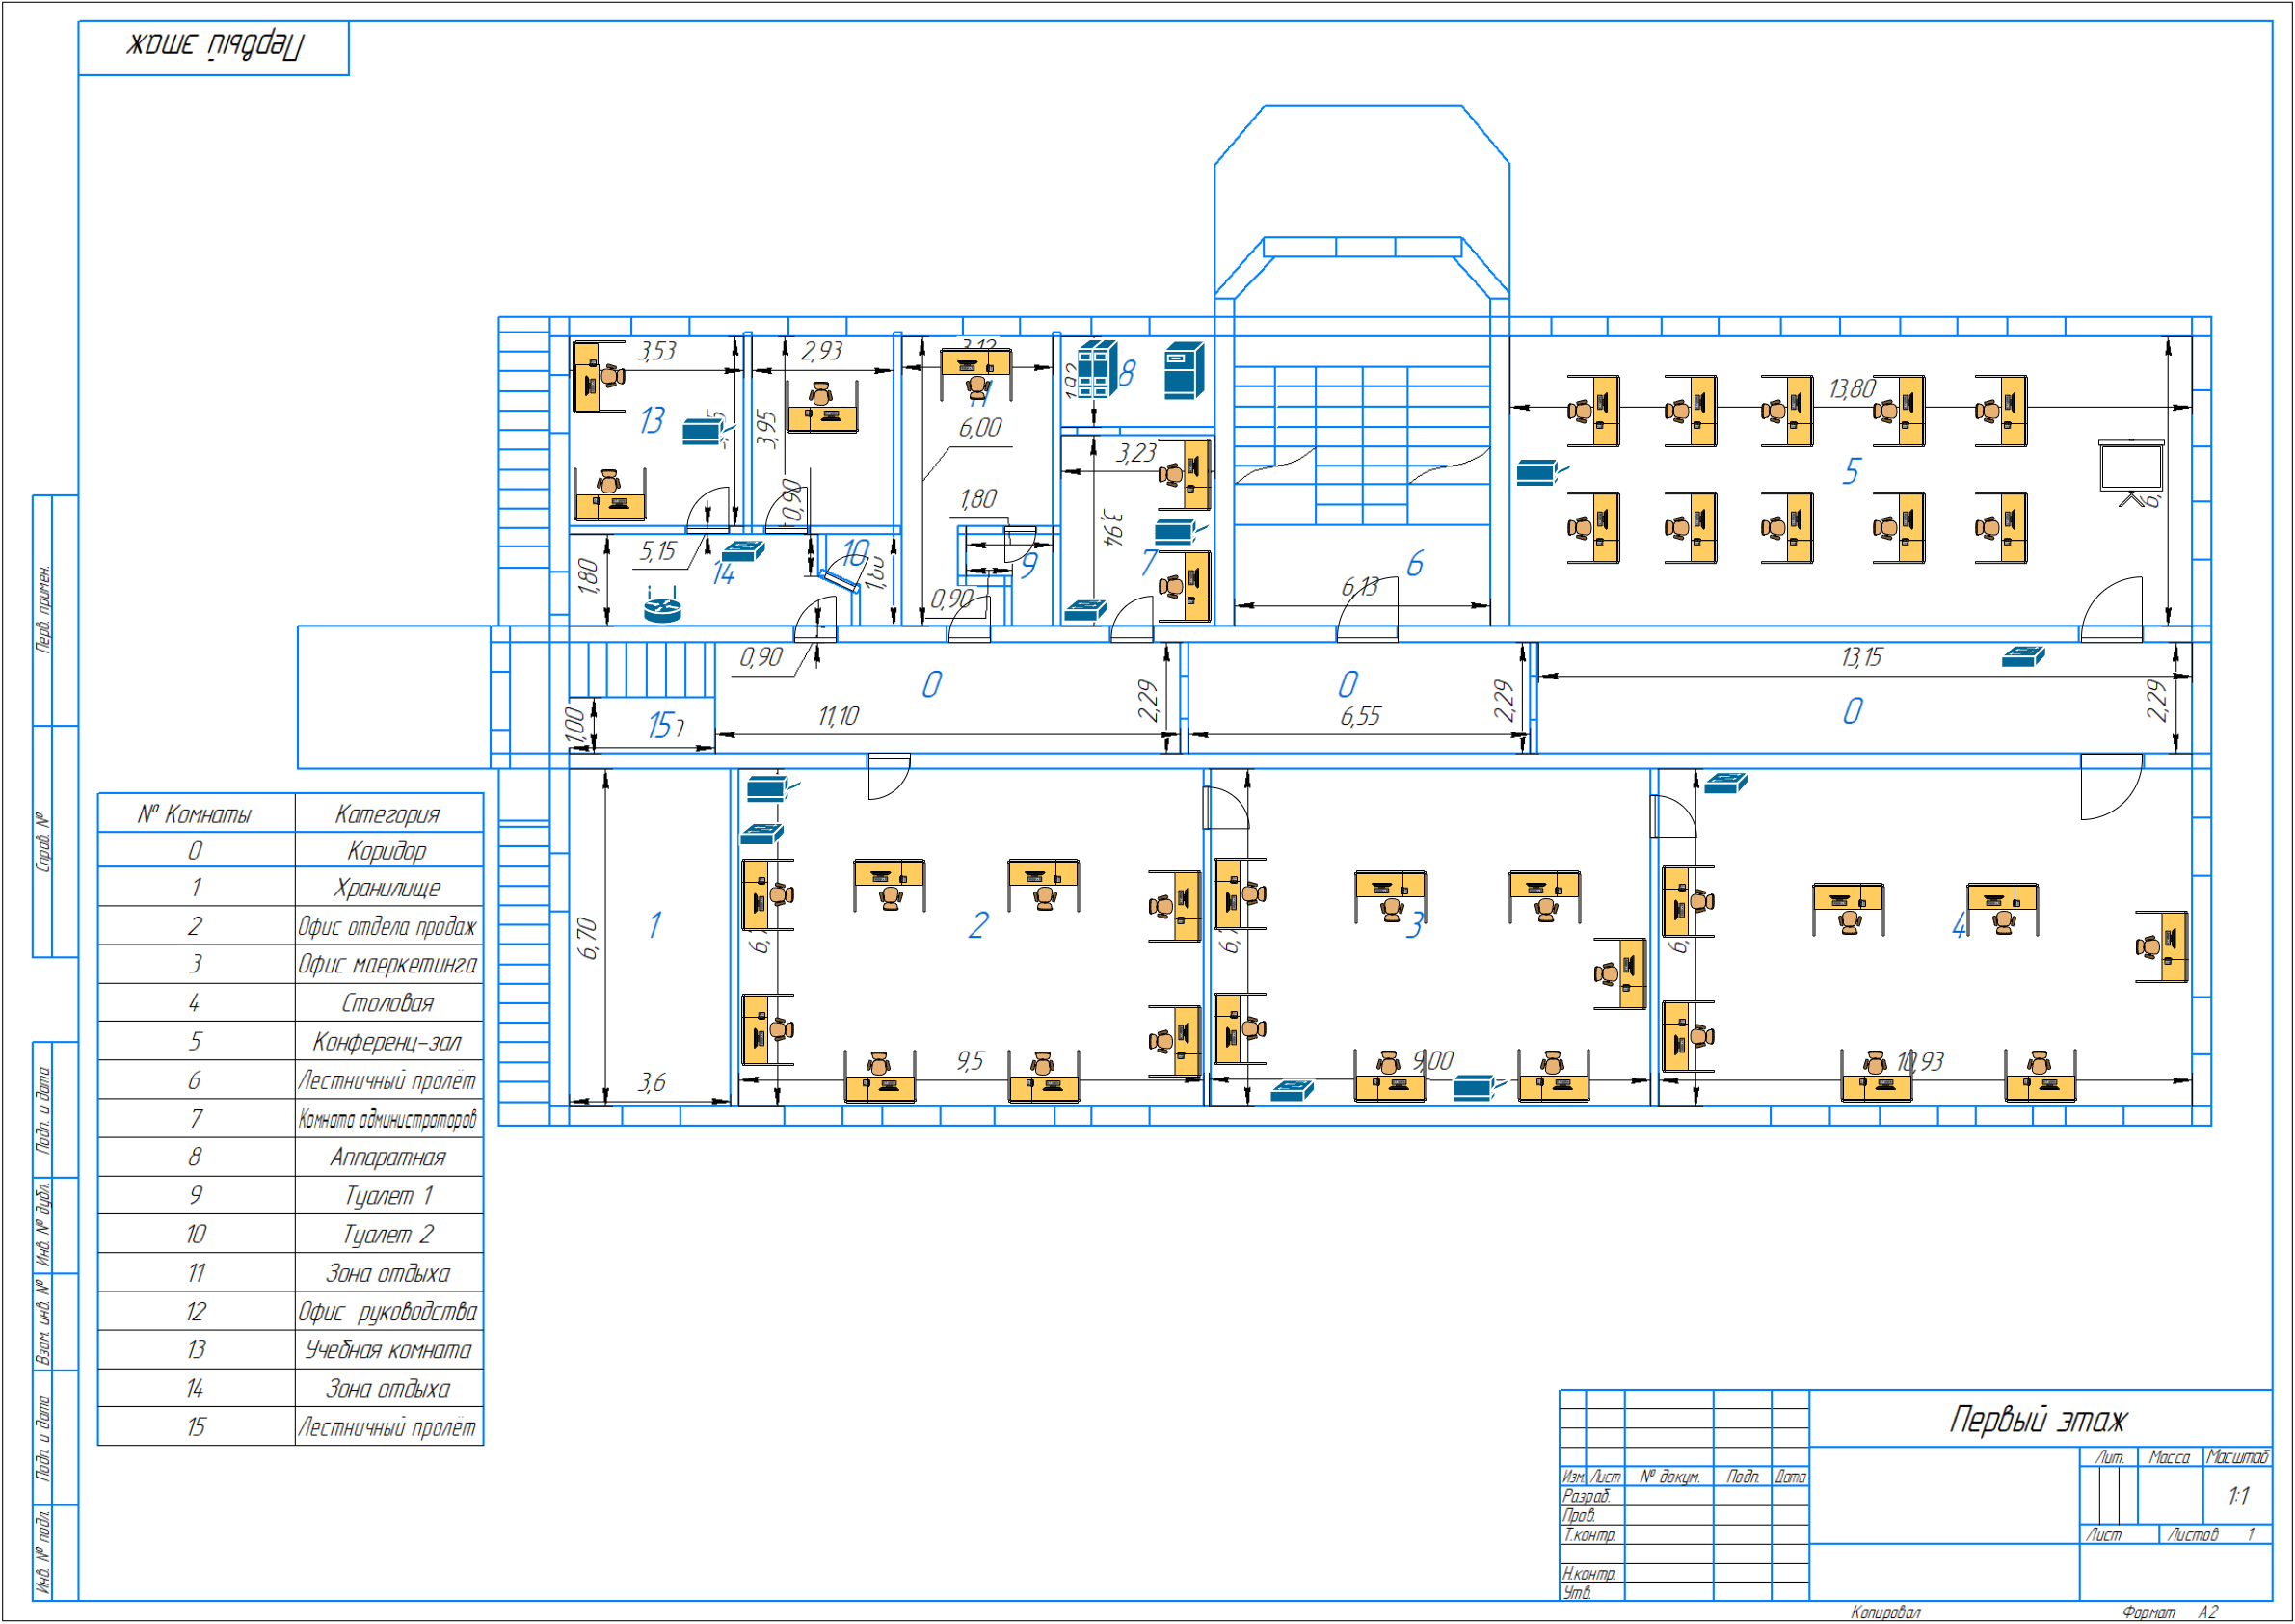
\includegraphics[width=\linewidth]{images/Схема по курсовому(2 этаж).png}
			\text Второй этаж
		\end{column}
	\end{columns}
\end{frame}

\begin{frame}{Рабочие места}
	\begin{block}{\large Группы пользователей}
	\vspace{0.1cm}
		\begin{itemize}
			\setlength{\leftmargin}{1.5cm}
			\setlength{\itemindent}{0.5cm}
			\setlength{\itemsep}{0.3cm}
			
			\item Зона отдыха и обучения
			\item Сеть инженерного отдела
			\item Сеть офиса отдела продаж
			\item Сеть офиса маркетинга.
			\item Конференц-зал
		\end{itemize}
	\end{block}
\end{frame}

\begin{frame}{Теоретико-графовая модель}
	\centering
	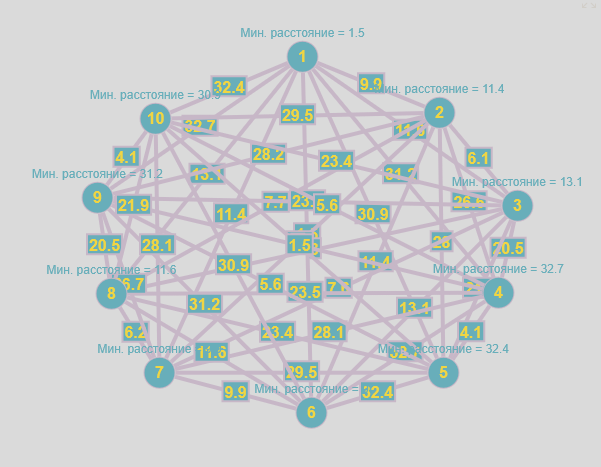
\includegraphics[width=0.7\linewidth]{images/Теоретико-графовая модель.png}
\end{frame}

\begin{frame}{Расстояния между точками}
	\centering
	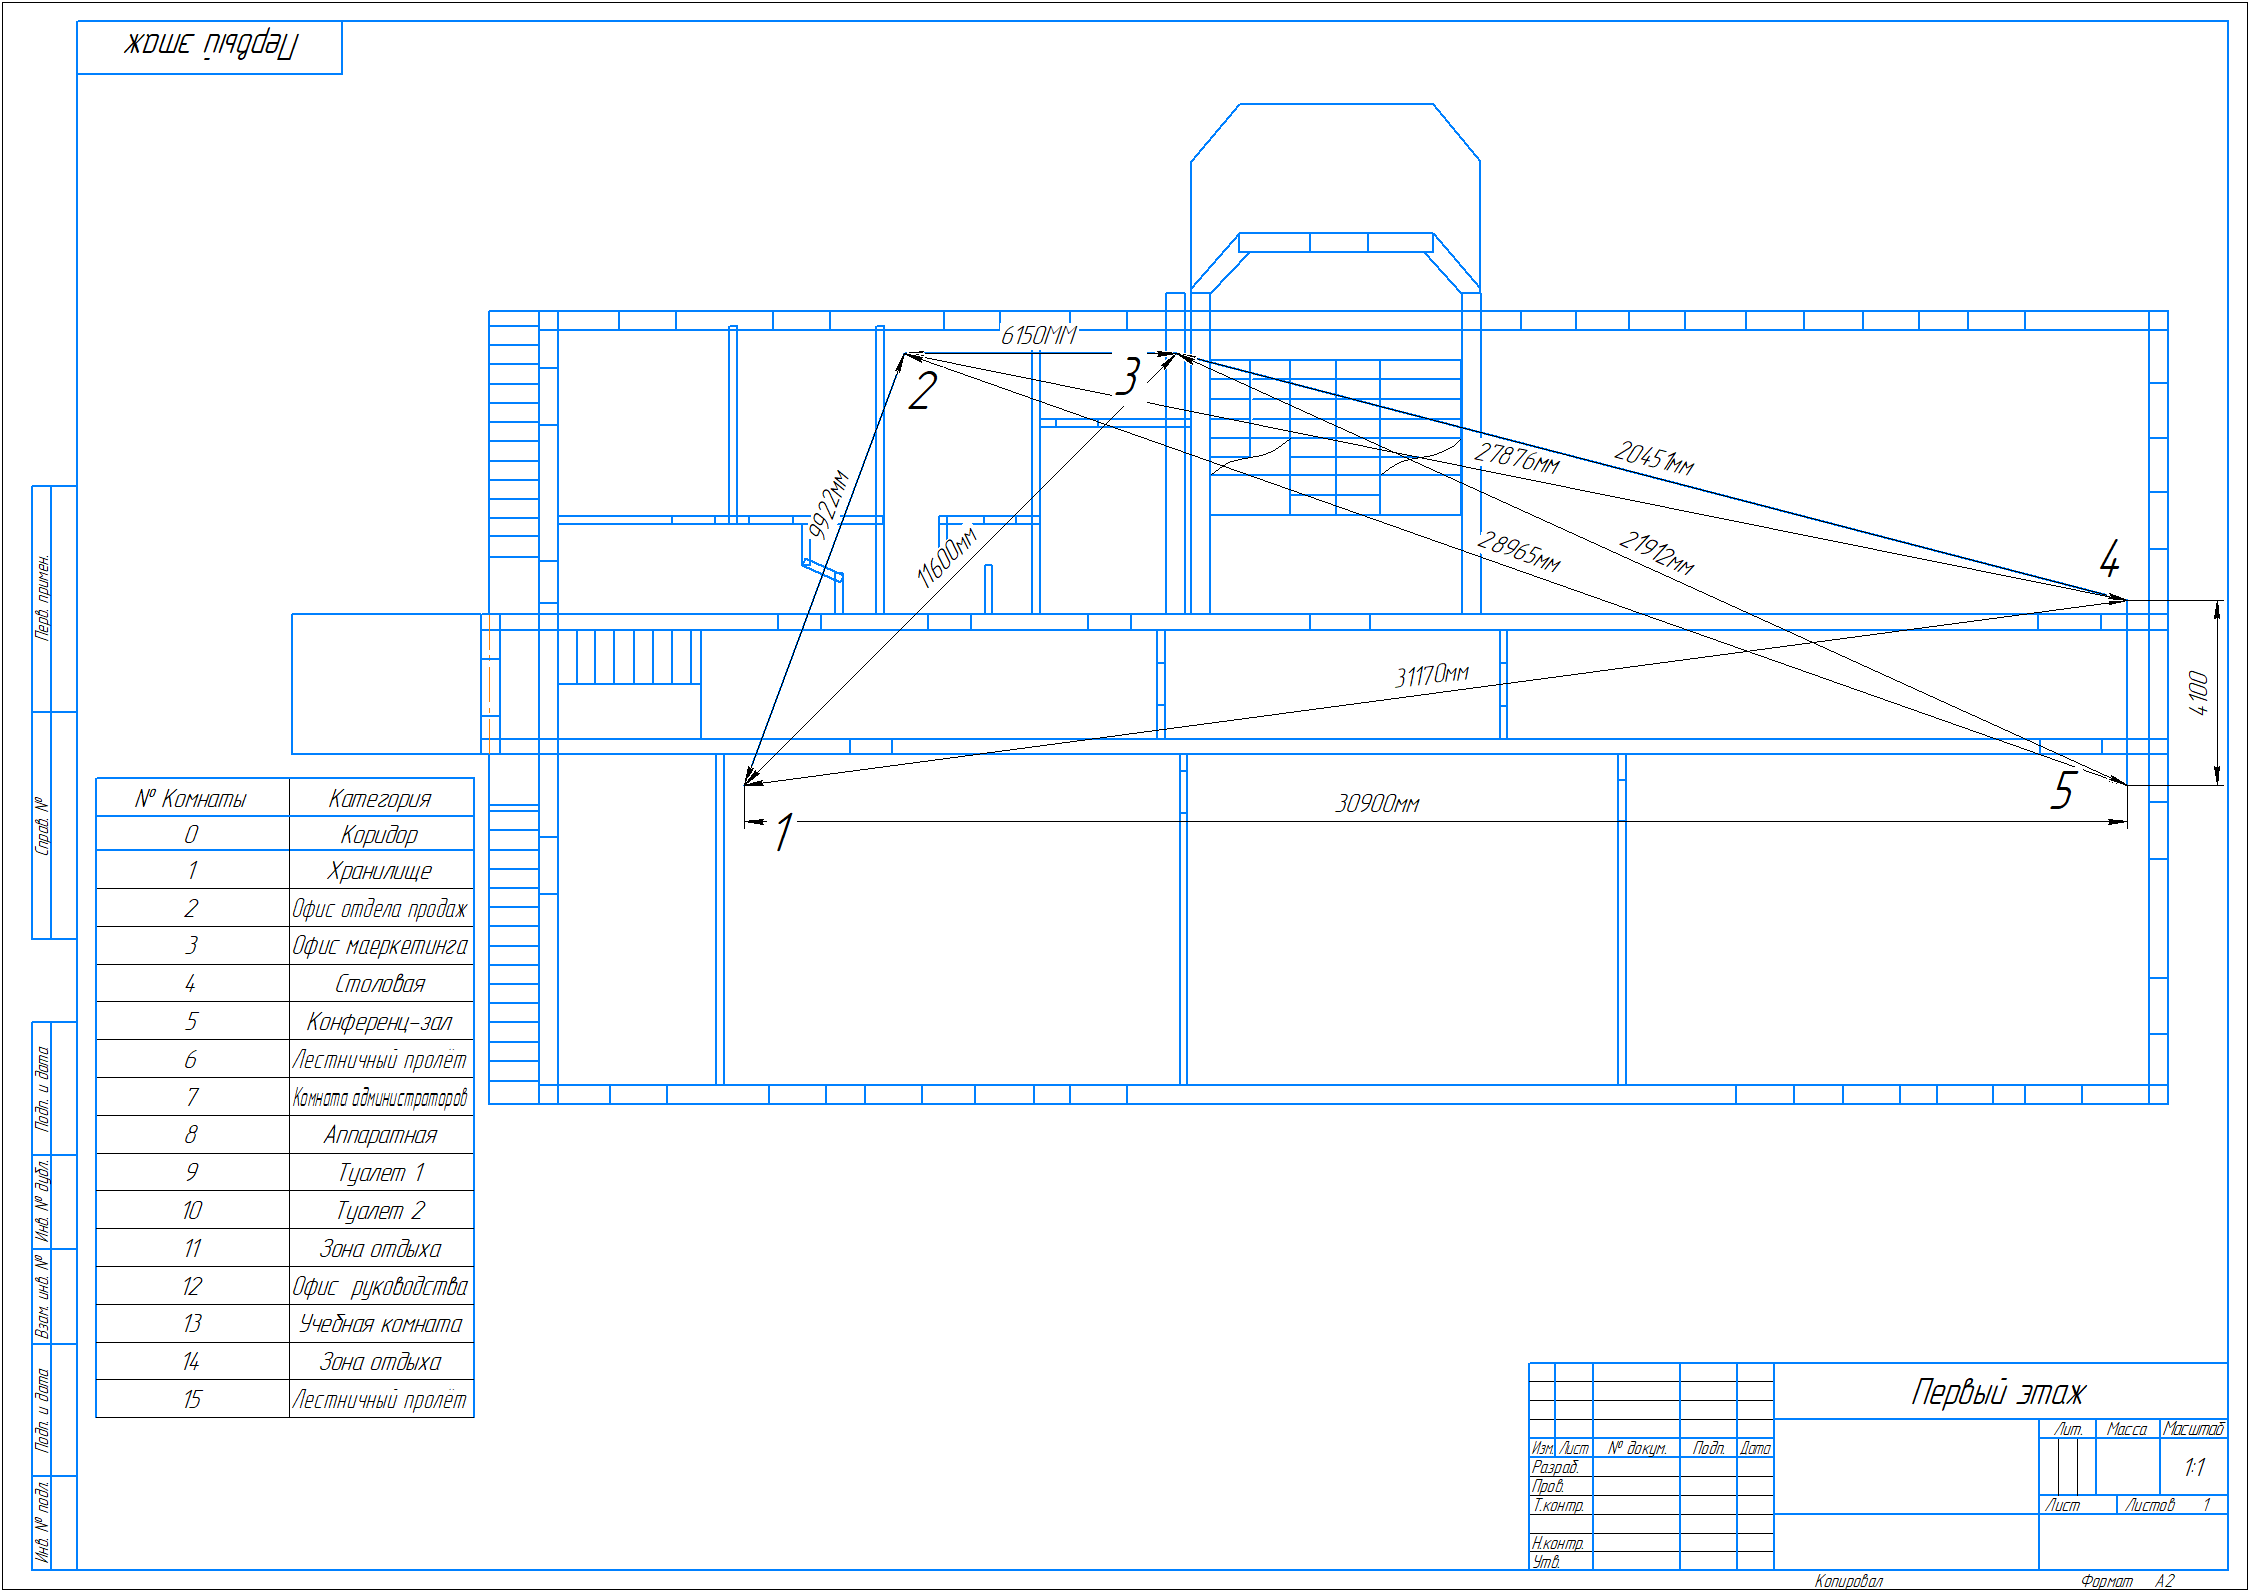
\includegraphics[width=0.7\linewidth]{images/Полная схема для расчётов(1 этаж).png}
\end{frame}

\begin{frame}{Центры графа}
	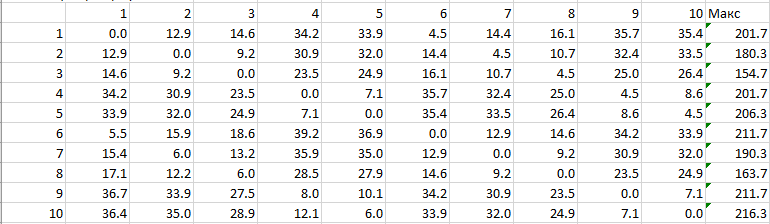
\includegraphics[width=\linewidth]{images/Центры графа.png}
\end{frame}

\begin{frame}{Логическое моделирование}
	\begin{tabular}{|p{0.4\textwidth}|p{0.5\textwidth}|}
		\hline
		\vspace{0.4cm}
		\centering
		\text{Уровень ядра} & 
		\vspace{0.01cm}
		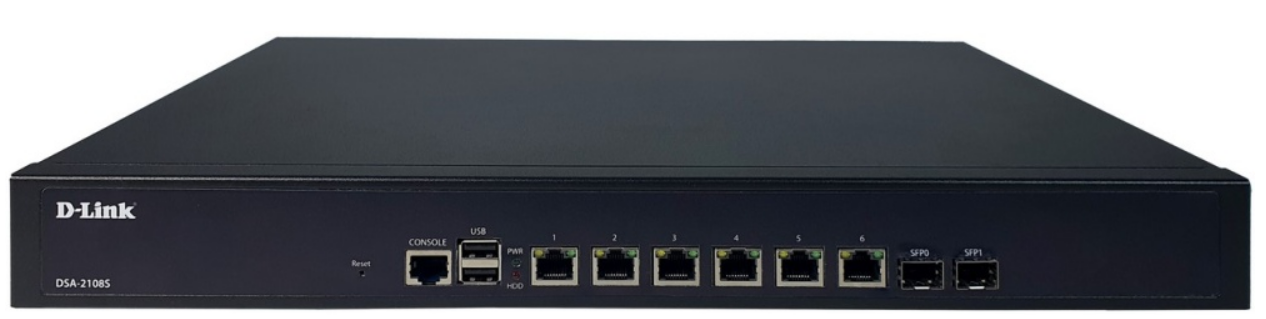
\includegraphics[width=4.8cm,height=4cm,keepaspectratio]{images/Маршрутизатор.png} \\
		& \footnotesize Маршрутизатор D-Link DSA-2108S  \\
		\hline
		
		\hline
		\vspace{0.4cm}
		\centering
		\text{Уровень распределения} & 
		\vspace{0.01cm}
		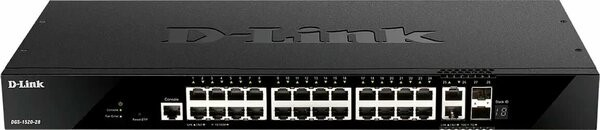
\includegraphics[width=4.8cm,height=4cm,keepaspectratio]{images/Коммутатор L3.jpg} \\
		& \footnotesize Коммутатор L3 D-Link DGS-1520-28 \\
		\hline
		
		\hline
		\vspace{0.4cm}
		\centering
		\text{Уровень доступа} & 
		\vspace{0.01cm}
		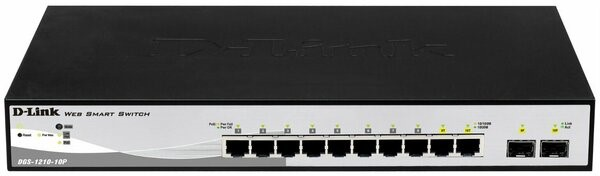
\includegraphics[width=4.8cm,height=4cm,keepaspectratio]{images/Коммутатор L2.jpg} \\
		& \footnotesize Коммутатор L2 D-Link DGS-1210-10 \\
		\hline
  \end{tabular}
\end{frame}

\begin{frame}{Прокладка кабеля}
	\centering
	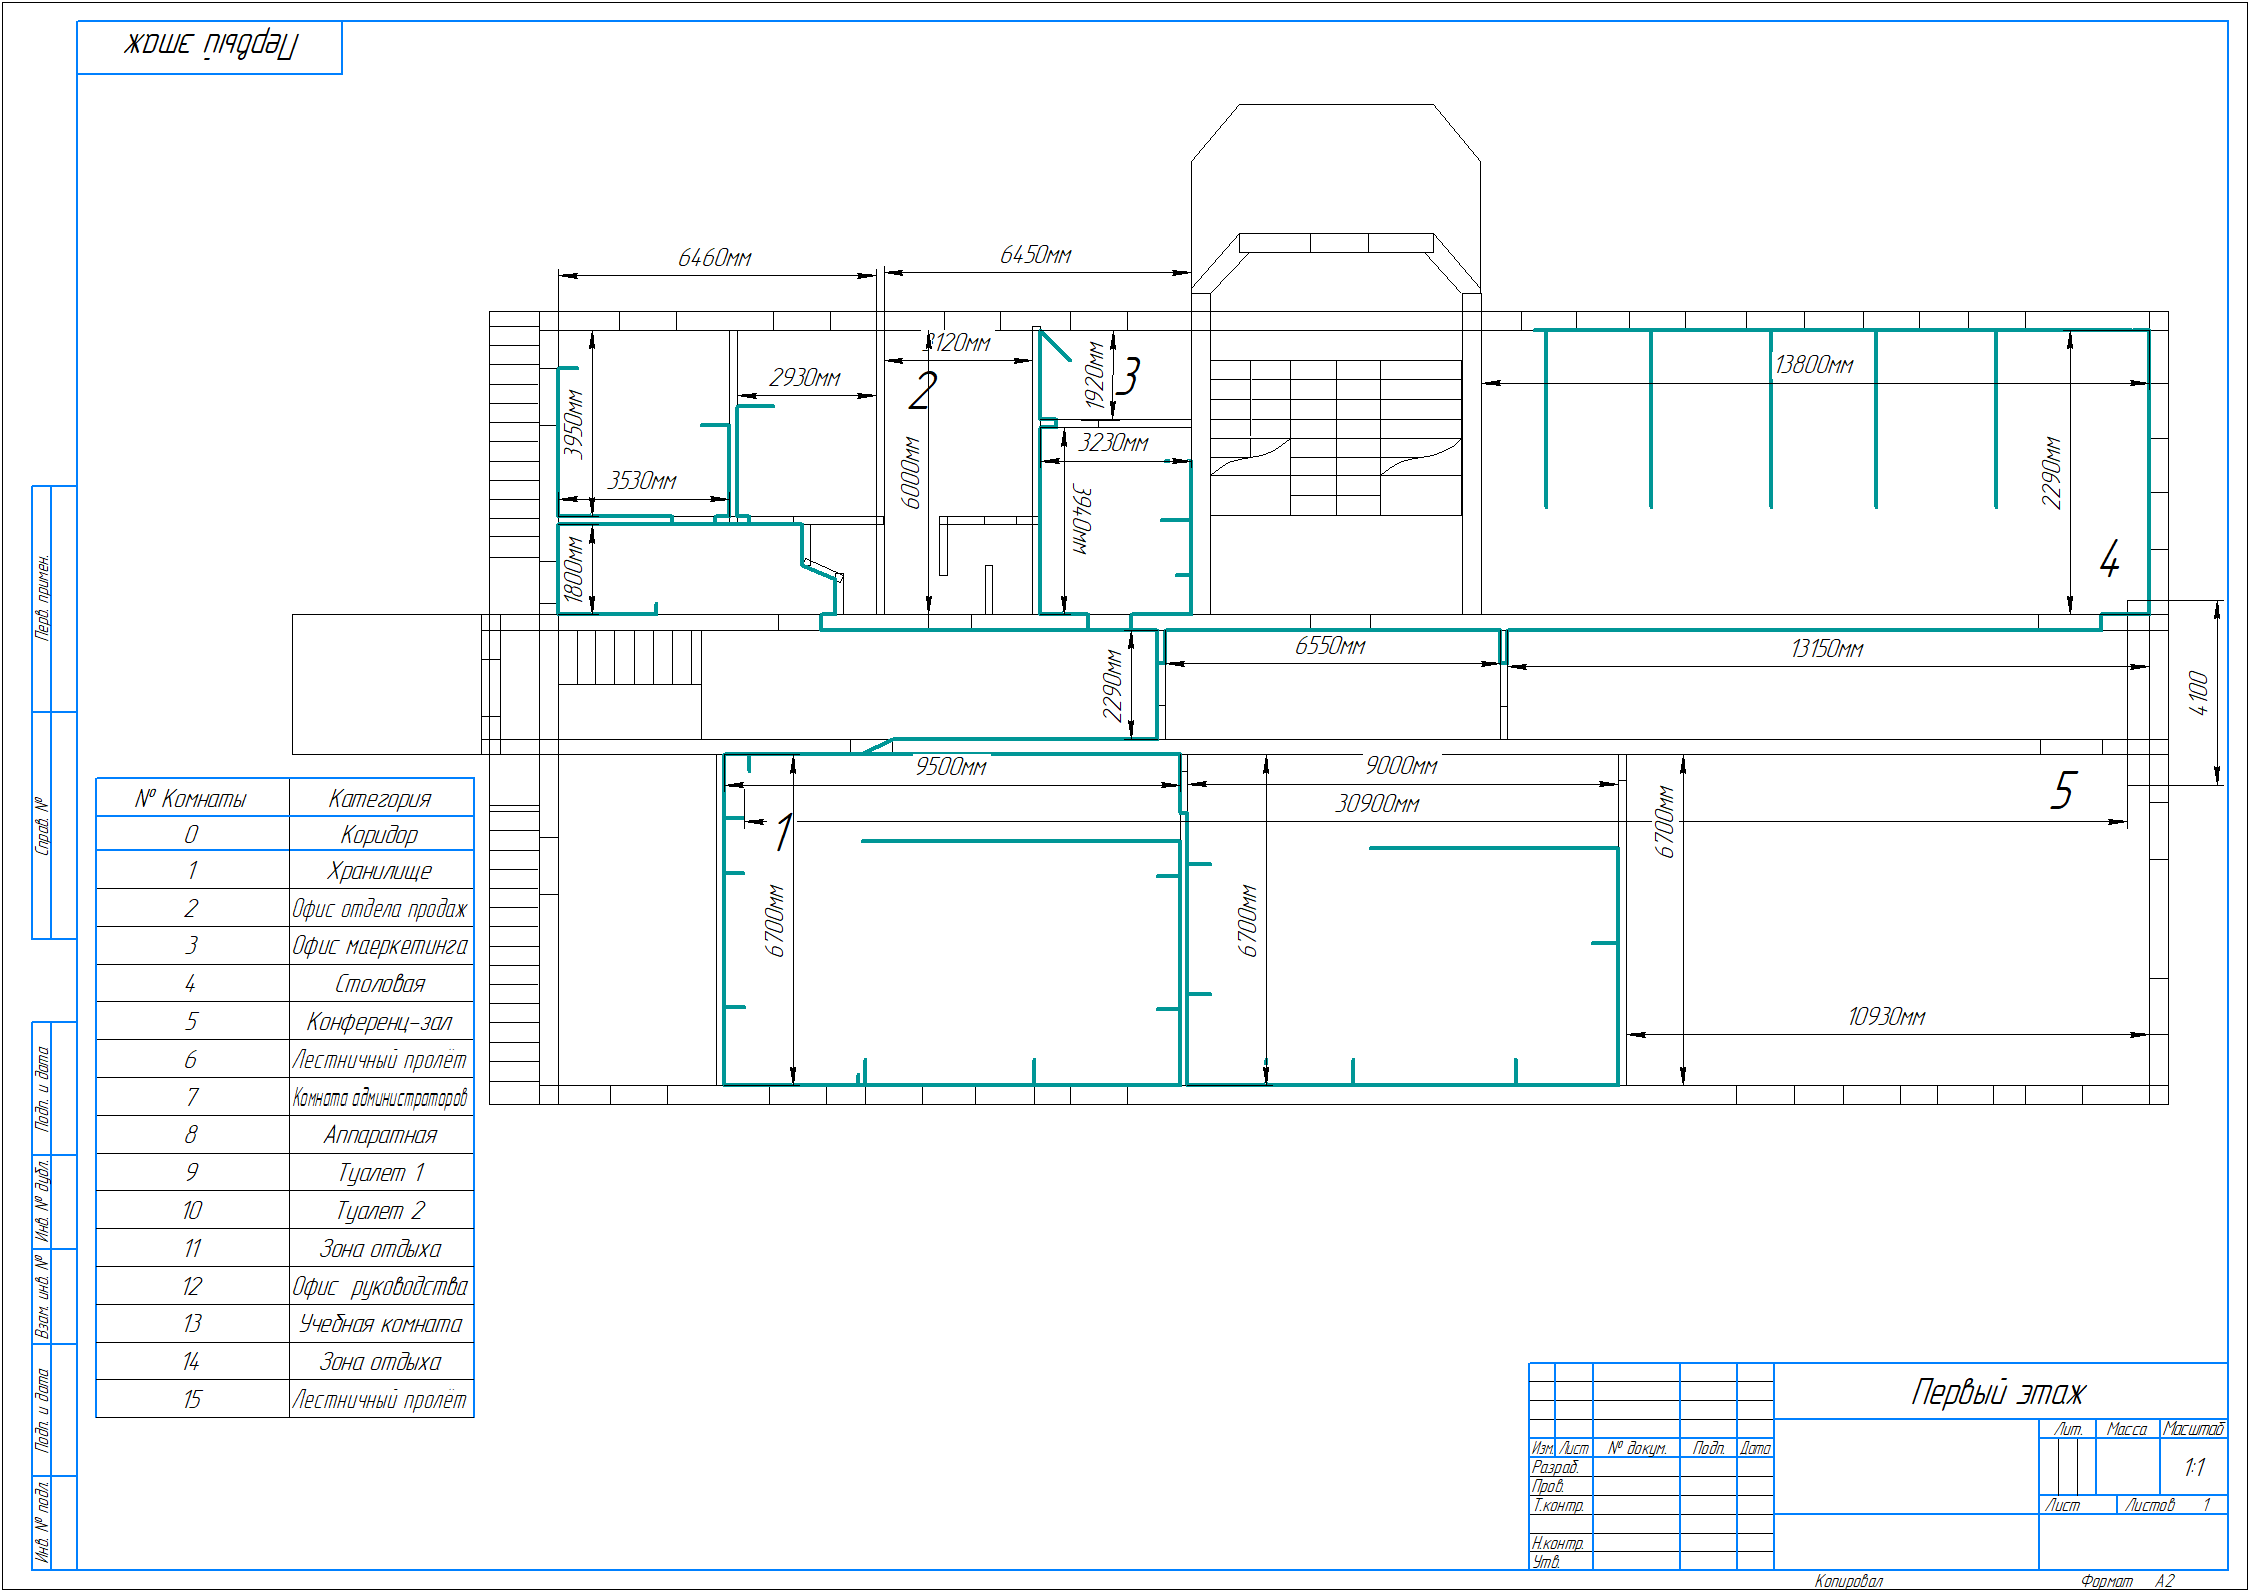
\includegraphics[width=0.8\linewidth]{images/Полная схема для расчётов длины кабеля.png}
\end{frame}

\begin{frame}{Внутренности коммутационного шкафа}
	\centering
	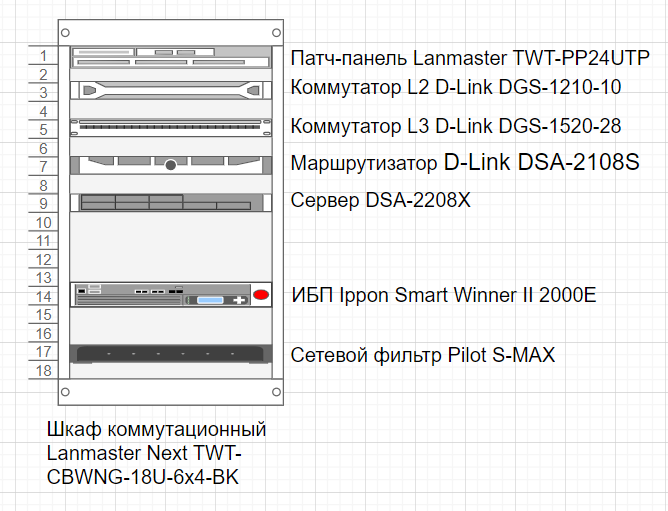
\includegraphics[width=0.6\linewidth]{images/Коммутационный шкаф.png}
\end{frame}

\begin{frame}{Экономические расчёты}
	\centering
	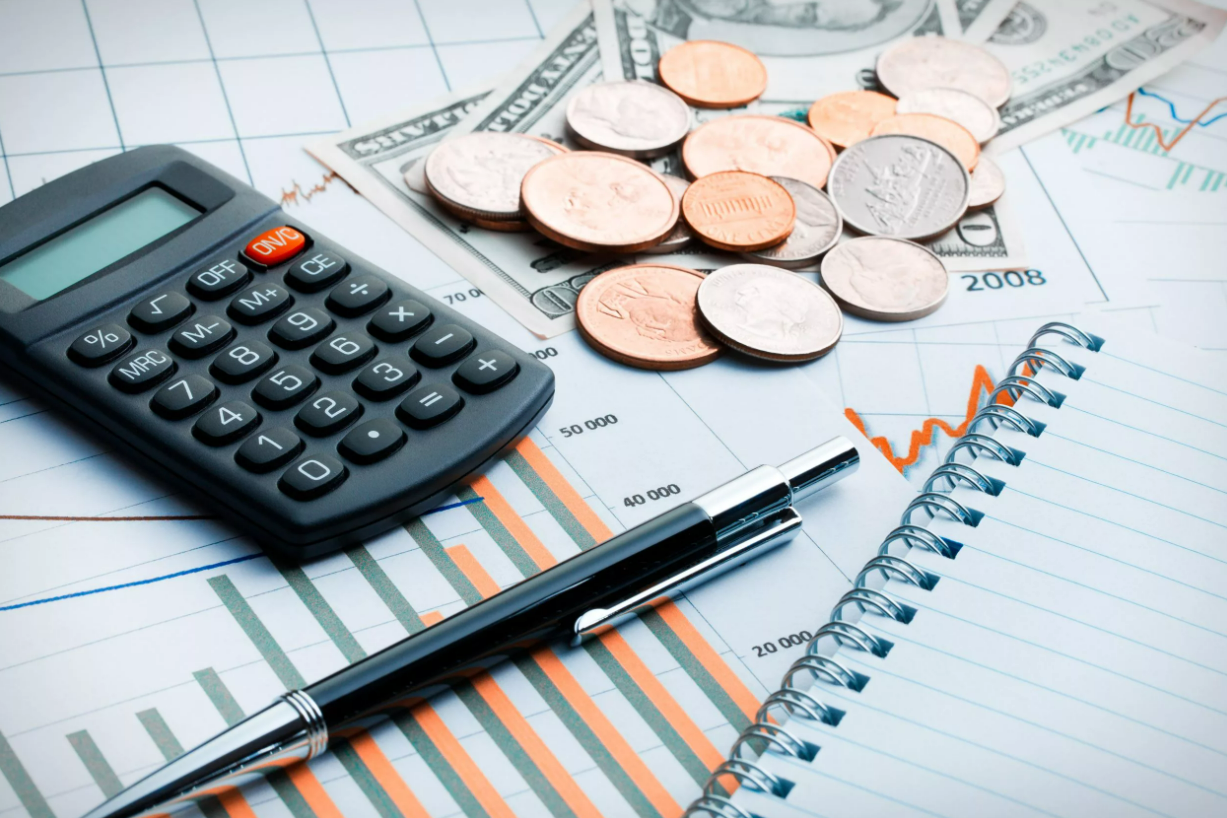
\includegraphics[width=0.7\linewidth]{images/Экономические расчёты.png}
\end{frame}

\begin{frame}{Активное оборудование}
	\centering
	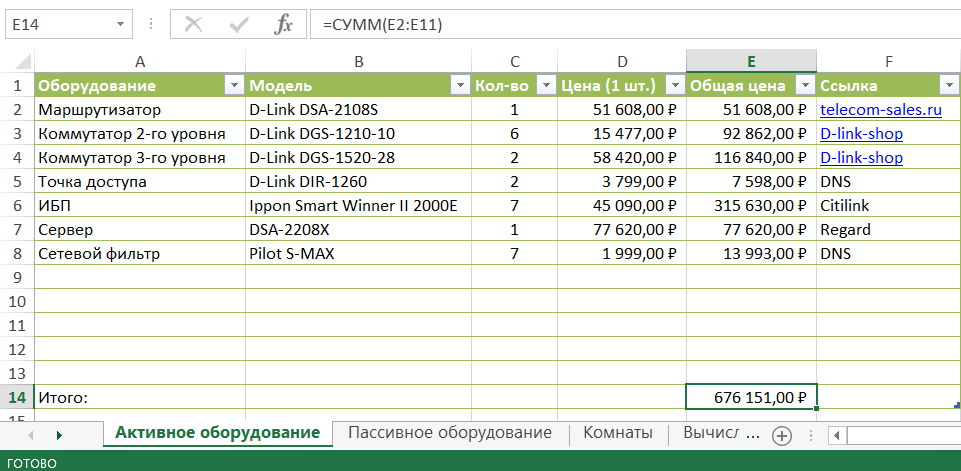
\includegraphics[width=\linewidth]{images/Активное оборудование.png}
\end{frame}

\begin{frame}{Пассивное оборудование}
	\centering
	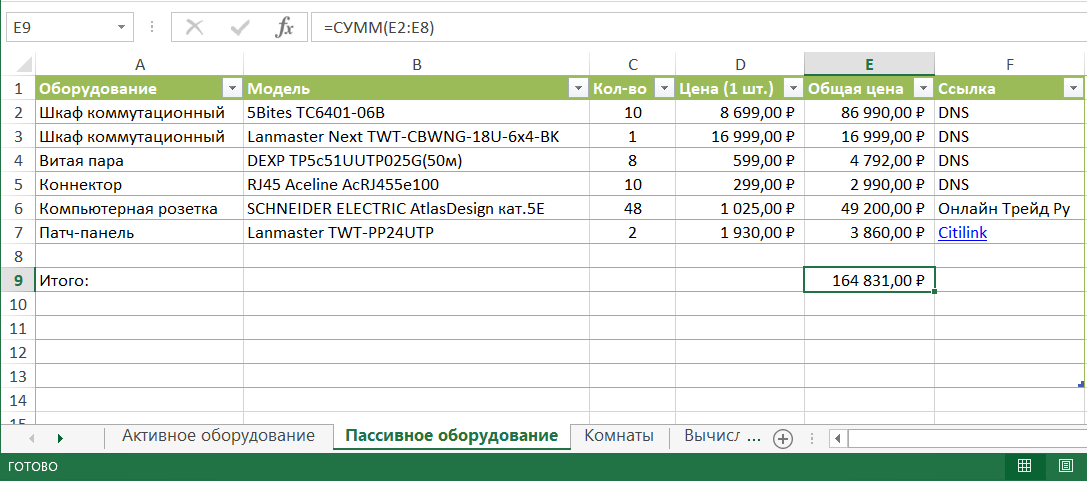
\includegraphics[width=\linewidth]{images/Пассивное оборудование.png}
\end{frame}

\begin{frame}{Общая стоимость}
	\centering
	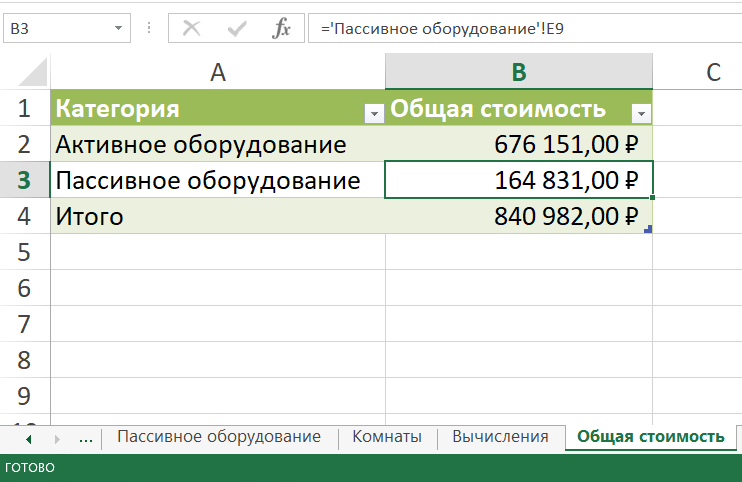
\includegraphics[width=0.8\linewidth]{images/Общая сумма.png}
\end{frame}

\begin{frame}
	\begin{center}
		\huge Спасибо за внимание!
	\end{center}
\end{frame}

\end{document}
